\subsection{QuizziPedia::Back-End::App}
\subsubsection{Informazioni generali}
\label{QuizziPedia::Back-End::App}
\begin{figure}
	\centering
	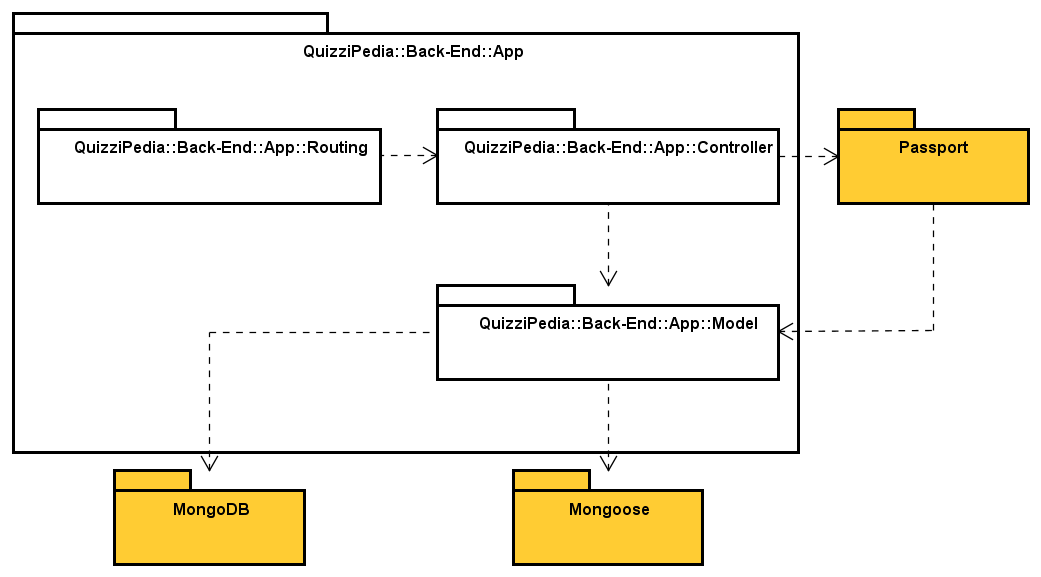
\includegraphics[scale=0.45]{UML/Package/QuizziPedia_Back-End_App.png}
	\caption{QuizziPedia::Back-End::App}
\end{figure}
\FloatBarrier
	\begin{itemize}
		\item \textbf{Descrizione} \\
		Package\ped{G} contenente le componenti del server\ped{G} che implementano il \textit{pattern\ped{G} MVC\ped{G}};
		\item \textbf{Padre} \texttt{Back-End}
		\item \textbf{Interazioni con altri componenti}
			\begin{itemize}
				\item Config \\
				Package contenente le componenti di configurazione del server\ped{G}.
			\end{itemize}
		\item \textbf{Package contenuti}
			\begin{itemize}
				\item Controllers \\
				Package\ped{G} che contiene i controllers di Express\ped{G}, definisce la logica dell'applicazione;
				\item Models \\
				Package\ped{G} che contiene le classi che definiscono il model dell'applicazione. Queste classi cono definite come classi schema di Mongoose\ped{G}, il quale permette di utilizzare MongoDB\ped{G} tramite degli oggetti;
				\item Routers \\
				Package\ped{G} contenente i routers della componente back-end dell'applicazione. Contiene i file di configurazione relativi al routing delle richieste del client\ped{G}, ossia i routers di Express\ped{G}.
			\end{itemize}
	\end{itemize}